\chapterimage{ChapterCover.pdf} % Chapter heading image
\chapter{Linear Mixed-Effects Models (LMM)}

\epigraph{\textit{cool quote about LMM.}}{\rightline{{\rm --- \href{https://en.wikipedia.org/wiki/Marvin_Minsky}{some philosopher}}}}

\minitoc
\newpage
\section{Background: Introduction to Statistical Modeling}
In many fields of research, from psychology and education to medicine and social sciences, the primary goal is to understand and explain relationships between variables. Often, researchers collect data that involves complex relationships, where outcomes (dependent variables) are influenced by several factors (independent variables). Statistical modeling provides the tools needed to quantify these relationships, identify patterns, and make predictions based on data. Without a structured approach to data analysis, researchers risk making inaccurate conclusions, or even worse, overlooking important relationships that could drive insights or interventions.

At its core, statistical modeling is a way of representing data through mathematical equations, allowing researchers to describe, explain, and predict real-world phenomena. These models help simplify complex systems by providing a framework for analyzing the effects of multiple variables simultaneously, while also accounting for random variation and uncertainty. For example, in psychology, statistical models are used to examine how different cognitive, emotional, or environmental factors influence behavior. In education, models might be used to study how teaching methods or school environments affect student performance. In medicine, researchers might use statistical models to identify factors that influence the progression of a disease or the effectiveness of a treatment. And in social sciences, models can help understand complex social behaviors and the impact of policy changes or societal trends.

In each of these fields, the challenge is often that data is not independent or identically distributed. Real-world data frequently comes with some form of hierarchy or clustering — for instance, multiple measurements from the same individual over time, or students nested within different schools. This means that the observations in a dataset are not independent of each other, violating the assumptions of traditional statistical methods, such as ordinary least squares regression. As a result, more sophisticated modeling techniques are needed to properly account for these complex data structures and avoid biased or misleading conclusions. This is where models like linear mixed-effects models (LMM) become invaluable, as they offer a way to include both fixed effects (representing population-level relationships) and random effects (accounting for individual or group-level variability).

Statistical models thus serve as a powerful tool in research by transforming raw data into insights. These models can reveal patterns and associations that might not be immediately obvious, test hypotheses, control for confounding factors, and enable researchers to make inferences about larger populations based on sample data. As datasets continue to grow in size and complexity, the need for robust, flexible, and accurate statistical modeling has never been greater. Linear mixed-effects models represent one such advancement, allowing for a more nuanced understanding of how various factors affect outcomes in hierarchical or grouped data structures.

\subsection*{Limitations of Simple Linear Models}
Traditional linear models, such as ordinary least squares (OLS) regression, have long been the foundation for statistical analysis due to their simplicity and interpretability. These models assume that the relationship between the independent variables (predictors) and the dependent variable (outcome) is linear, and that all observations in the dataset are independent of each other. Under these assumptions the dependent variable can be expressed as a weighted sum of the independent variables, plus an error term:
\[
y_i = \beta_0 + \beta_1 x_i + \epsilon_i
\]

\noindent Where:
\begin{itemize}
\item $y_{i}$ is the dependent variable (response) for observation $i$
\item $x_{i}$ is the independent variable (predictor)
\item $\beta_0$  is the intercept (value of $y$ when $x=0$)
\item $\beta_1$ is the slope (change in $y$ for a one-unit change in $x$)
\item $\epsilon_i$ is the error term (random deviation)
\end{itemize}

Multiple independent variables are possible too in this context. In multiple linear regression, we simply have $n$ more predictors:
\[
y_i = \beta_0 + \beta_1 x_{i1} + \beta_2 x_{i2} + ... \beta_n x_{in} + \epsilon_i
\]

 The goal of OLS is to find the values of $\beta_0, \beta_1, \beta_2, ... \beta_n$ that minimize the sum of squared residuals (SSR). A residual is the difference between the observed value $y_i$ and the predicted value $\hat{y}_i$.
 
 So, OLS minimizes:
 \[
SSR=\sum_{i=1}^{n}(y_i - \hat{y}_i)^2
\]

This is why it's called ``least squares'': it finds the line (or hyperplane in multiple regression) that minimizes the squared distance from each data point to the regression line.

 OLS regression works well when the data points are independent and identically distributed, and when there is no clustering or grouping of observations. However, this idealized scenario is rare in real-world data, especially in fields like psychology, education, medicine, and social sciences, where nested or hierarchical data structures are common.

In many research designs, data are inherently grouped. For example, in a longitudinal study of patients, multiple measurements are taken from the same individuals over time, creating repeated observations within each subject. Similarly, in educational research, students are nested within schools, and observations from students in the same school are likely to be more similar to one another than to students from different schools. This hierarchical structure introduces two key sources of variability that traditional linear models fail to account for: within-group variability (differences among individuals within the same group) and between-group variability (differences between groups themselves).

The standard OLS model assumes that all data points are independent, which is violated in these hierarchical structures. When this assumption is not met, the model's estimates of regression coefficients can become biased or inefficient, leading to inaccurate conclusions. Specifically, by ignoring the clustering of data, the model treats all observations as if they are equally independent, which underestimates the true variability in the data. This often results in incorrect standard errors, leading to misleading significance tests and inflated Type I error rates (false positives). In other words, the model may indicate that certain relationships are statistically significant when, in fact, they may be due to the unaccounted-for correlation between observations within the same group.
Furthermore, OLS regression cannot properly model the variability between groups. For instance, when multiple groups (e.g., schools, hospitals, or geographic regions) are involved, the assumption that all subjects respond the same way to predictors becomes unrealistic. Some schools may have inherently better academic outcomes due to local factors, and this variation needs to be explicitly modeled. Without accounting for this group-level variability, the OLS model does not allow for differences in intercepts or slopes between groups, thus simplifying the model to an unrealistic assumption that one set of coefficients applies universally across all levels of the data.

The result of using a simple linear model on nested data is not only potential bias in estimates but also a loss of the ability to capture the complexities inherent in the data structure. This is where linear mixed-effects models (LMMs) provide an important advantage. By incorporating random effects to account for variability within and between groups, mixed-effects models offer a more flexible and accurate way to model hierarchical data, providing a better understanding of how predictors influence outcomes at both the individual and group levels.

\section{The Need for Mixed-Effects Models}
\subsection*{Fixed vs. Random Effects}
In the context of linear mixed-effects models (LMMs), one of the key features is the distinction between fixed effects and random effects. These two types of effects allow researchers to model both the population-level relationship between predictors and the response variable, as well as the variability among groups or individuals that cannot be captured by fixed effects alone.

\subsubsection{Fixed Effects: Population-Level Relationships}
Fixed effects represent the systematic, population-level relationship between the predictors (independent variables) and the response variable (dependent variable). These effects are constant across all levels of the grouping factor and are typically used to estimate the average effect of a treatment or intervention, or the overall relationship between a predictor and the outcome. For example, in a study where the effect of a new teaching method on student performance is assessed, the fixed effect for the teaching method would represent the average difference in performance between the treatment group and the control group, across all students. This effect is the same for all individuals or groups in the dataset, and it reflects the population-level trend that one expects to see on average.

In a simple linear regression model, all coefficients are considered fixed effects. In mixed-effects models, the fixed effects still represent the population-level effects, but they are combined with random effects to account for variability at different levels of the data hierarchy. For example, in a multilevel model examining students' test scores, fixed effects could include predictors like the student's age, gender, or teaching method, which are expected to have the same effect for every student across all schools.

Mathematically, the fixed effect coefficients ($\beta_0,\beta_1, \dots$) are typically estimated from the data using methods like maximum likelihood estimation (MLE) or restricted maximum likelihood estimation (REML). These fixed effects are what we are most interested in when trying to understand the general trends or relationships in the data that apply across the entire population.

\subsubsection*{Random Effects: Group-Level and Individual-Level Variability}
In contrast to fixed effects, random effects account for variability at the group or individual level. These effects capture the fact that different groups or individuals may respond differently to the same treatment or exposure. For instance, even if a new teaching method has an average positive effect on students' performance (captured by the fixed effect), some students might show a much stronger response, while others might show a weaker or even negative response. This variation among individuals, or among groups (such as schools), is modeled as random effects.

In a typical mixed-effects model, random effects are included to model the variation in the intercept (random intercepts) or the variation in the slopes (random slopes) across groups or individuals. For example, in a longitudinal study of patient outcomes, the response variable might be influenced by both a fixed effect (e.g., treatment) and a random effect (e.g., individual patient differences). Random intercepts would allow each patient to have their own baseline level of the outcome variable, accounting for the fact that some patients start with higher or lower values. Random slopes could be included if the treatment effect varies across individuals, meaning some patients might benefit more from the treatment than others.

Mathematically, random effects are often represented as deviations from the overall fixed effect, where the random effect term ($u_j$) is assumed to follow a normal distribution with a mean of zero and a variance of $\sigma_u^2$. These random effects are estimated along with the fixed effects and provide a way of partitioning the variance in the response variable into components that reflect both systematic effects (fixed) and individual or group-level variability (random).

\subsubsection*{Fixed vs. Random Effects: Complementary Roles}
The distinction between fixed and random effects is essential for understanding the full range of variation in the data. Fixed effects tell us about the overall trend in the data, such as the effect of a treatment, whereas random effects tell us about the individual differences in how subjects or groups respond to that treatment. Together, they offer a more complete and nuanced understanding of the data, allowing for more accurate predictions and insights.

\begin{figure}[ht]
\centering
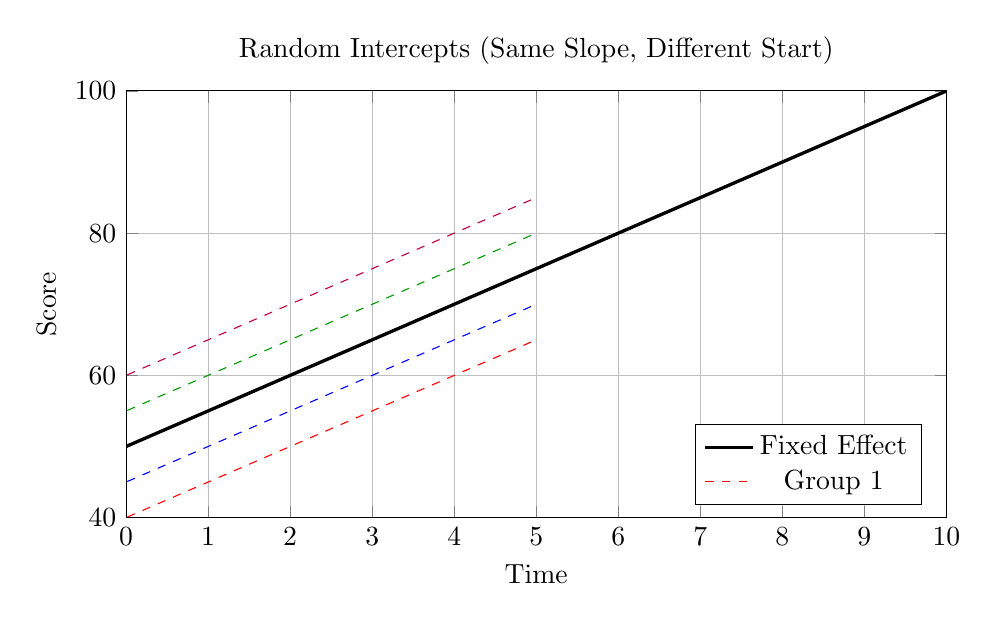
\begin{tikzpicture}
  \begin{axis}[
    xlabel=Time,
    ylabel=Score,
    title={Random Intercepts (Same Slope, Different Start)},
    legend pos=south east,
    xmin=0, xmax=10,
    ymin=40, ymax=100,
    width=12cm, height=7cm,
    grid=both,
  ]

  \addplot[very thick, black, domain=0:10] {5*x + 50};
  \addlegendentry{Fixed Effect}

  \addplot[dashed, red] {5*x + 40}; \addlegendentry{Group 1}
  \addplot[dashed, blue] {5*x + 45};
  \addplot[dashed, green!60!black] {5*x + 55};
  \addplot[dashed, purple] {5*x + 60};

  \end{axis}
\end{tikzpicture}
\caption{Each group shares the same slope (fixed effect), but starts at a different baseline.}
\end{figure}

%--- RANDOM SLOPES ---
\begin{figure}[ht]
\centering
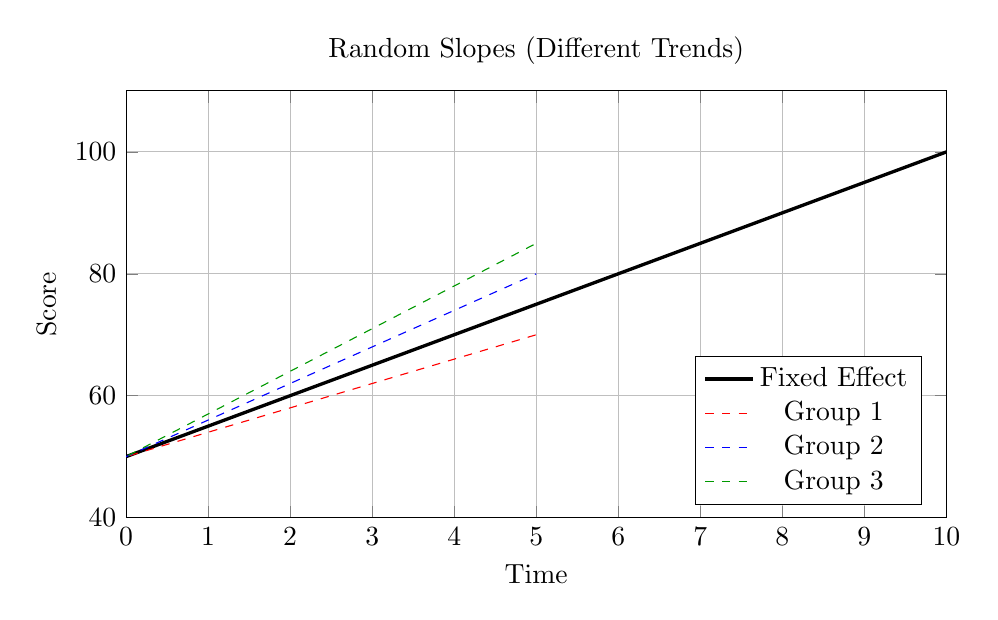
\begin{tikzpicture}
  \begin{axis}[
    xlabel=Time,
    ylabel=Score,
    title={Random Slopes (Different Trends)},
    legend pos=south east,
    xmin=0, xmax=10,
    ymin=40, ymax=110,
    width=12cm, height=7cm,
    grid=both,
  ]

  \addplot[very thick, black, domain=0:10] {5*x + 50};
  \addlegendentry{Fixed Effect}

  \addplot[dashed, red] {4*x + 50}; \addlegendentry{Group 1}
  \addplot[dashed, blue] {6*x + 50}; \addlegendentry{Group 2}
  \addplot[dashed, green!60!black] {7*x + 50}; \addlegendentry{Group 3}

  \end{axis}
\end{tikzpicture}
\caption{All groups start at the same baseline, but their rates of change differ.}
\end{figure}

%--- RANDOM INTERCEPTS + SLOPES + PREDICTIONS ---
\begin{figure}[ht]
\centering
\begin{tikzpicture}
  \begin{axis}[
    xlabel=Time,
    ylabel=Score,
    title={Random Intercepts and Slopes with Prediction Bands},
    legend pos=south east,
    xmin=0, xmax=10,
    ymin=30, ymax=120,
    width=12cm, height=7cm,
    grid=both,
  ]

  \addplot[very thick, black, domain=0:10] {5*x + 50};
  \addlegendentry{Fixed Effect (Population)}

  \addplot[dashed, red, name path=A] {4.5*x + 40}; \addlegendentry{Group 1}
  \addplot[dashed, blue, name path=B] {6.2*x + 52}; \addlegendentry{Group 3}

  % Shaded region between Group 1 and Group 3
  \addplot[gray!40, fill opacity=0.2] fill between[
    of=A and B,
    soft clip={domain=0:10}
  ];

  \end{axis}
\end{tikzpicture}
\caption{Combining both random slopes and intercepts, showing how predictions vary by group.}
\end{figure}


In many real-world datasets, observations are naturally organized into groups or clusters, creating a hierarchical structure. This means that the data are not independent of each other; rather, individual observations within a group are more similar to one another than to observations in other groups. Hierarchical data structures commonly arise in fields like education, medicine, and psychology, where subjects or units are nested within higher-level units. For instance, in an educational study, students are nested within classrooms, and classrooms are nested within schools. Similarly, in medical research, patients are nested within hospitals, and hospitals are nested within regions.

Hierarchical structures like these present unique challenges for statistical modeling, as traditional linear models assume that all observations are independent. Ignoring this clustering can lead to biased estimates and incorrect inferences. Linear mixed-effects models (LMMs) are designed to handle this kind of hierarchical data by explicitly modeling both fixed effects (population-level relationships) and random effects (group-level variability). In this framework, the data are divided into multiple levels, and the model accounts for the correlation within groups, while still allowing for variability between groups.

Consider a study examining student performance on a standardized test, where students are nested within classrooms, and classrooms are nested within schools. In this case, the data have three levels: individual students (Level 1), classrooms (Level 2), and schools (Level 3). A hierarchical model can accommodate this structure by including random effects for classrooms and schools, acknowledging that students within the same classroom or school may be more similar to each other than to students in other classrooms or schools.

For example, the fixed effects might include predictors such as study hours and parental involvement, representing the overall population-level effect on test scores. The random effects would capture the variability at the classroom and school levels. This means that while study hours might have a similar effect on students across all schools (captured by the fixed effect), there could be differences in how the effect of study hours is experienced at the classroom level, or how schools differ in their baseline student performance (captured by the random intercepts). A linear mixed-effects model would allow us to properly account for both the within-classroom and between-school variability, ensuring that we make accurate estimates of the treatment effects and group-level differences. By modeling the hierarchical structure in this way, mixed-effects models not only provide more accurate parameter estimates but also give us insights into how variability is distributed across different levels of the hierarchy, which is crucial for making valid conclusions in clustered data.

\section{Definition: Linear Mixed-Effects Models}
A linear mixed-effects model (LMM) is an extension of traditional linear regression that incorporates both fixed effects and random effects, allowing for more flexible modeling of data with hierarchical or grouped structures. While a standard linear regression model examines the relationship between one or more predictor variables and a response variable by estimating population-level coefficients, it assumes that the observations are independent and identically distributed. This assumption often fails when the data are nested or grouped, as is common in many real-world situations. To account for this, mixed-effects models introduce random effects, which model the correlation between observations within groups or clusters and allow for variability at multiple levels (e.g., individual, group, or time).

At its core, a linear mixed-effects model is similar to a linear regression model, but with the addition of random effects to capture the variability within and between groups. A typical linear regression model is specified as:
\begin{equation}
Y_i=\beta_0+\beta_1X_i+\epsilon_i 
\end{equation}

Where $Y_i$ is the response variable for observation $i$, $\beta_0$  is the intercept, $\beta_1$ is the coefficient for the predictor $X_i$, and $\epsilon_i$ is the error term representing residual variation. Note that this model assumes that all observations are independent and have the same error distribution.

In contrast, a linear mixed-effects model introduces random effects to account for clustering or grouping in the data. For example, in a study where multiple measurements are taken from individuals over time, a mixed-effects model would allow for each individual to have their own baseline (random intercept) and potentially a unique slope (random slope). The model can be written as:
\begin{equation}
Y_{ij}=\beta_0+\beta_1X_{ij}+\mu_j+\epsilon_{ij} 
\end{equation}

\noindent Where:
\begin{itemize}
\item $Y_{ij}$ is the response for observation $i$ within group $j$,
\item $\beta_0$ is the fixed intercept, representing the population-level average outcome when all predictors are zero,
\item $\beta_1$ is the fixed effect for the predictor $X_{ij}$,
\item $\mu_j$ is the random effect for group $j$, capturing the variation in the intercept across groups,
\item $\epsilon_{ij}$ is the residual error term for the individual observation, assumed to be independently distributed with zero mean and constant variance.
\end{itemize}

\subsection*{Fixed Effects vs. Random Effects}
The main distinction between fixed and random effects is their interpretation and role in the model:

Fixed effects represent the population-level relationship between the predictors and the outcome. These effects are assumed to be the same across all groups or individuals in the study. For example, in the model above, $\beta_0$ and $\beta_1$ are fixed effects, representing the overall intercept and the average effect of the predictor across all groups.

Random effects represent individual or group-level deviations from the overall trend captured by the fixed effects. These effects are unique to each group or individual and account for variability that cannot be explained by the fixed effects alone. In the model above, $u_j$ is a random intercept that allows each group to have its own baseline outcome, independent of the fixed intercept, $\beta_0$.

\subsubsection*{Why Use Mixed-Effects Models?}
Linear mixed-effects models are particularly useful when the data exhibit a hierarchical or clustered structure, such as repeated measures from the same individuals or measurements nested within groups. For instance, in a longitudinal study, measurements from the same subject over time are likely to be correlated, and using a simple linear regression would ignore this dependency, leading to biased estimates. By incorporating random effects, LMMs can model the correlation between repeated measurements from the same individual and provide more accurate and meaningful results.

Mixed-effects models also offer flexibility in modeling variability at multiple levels. For example, in a study of student performance across schools, random effects could model both the individual variation in performance (random intercepts) and the variation in how teaching methods affect different students (random slopes). This level of detail allows researchers to better understand not just the average effects of predictors, but also how those effects might vary across different contexts or groups.

\section{Assumptions About Random Effects in Linear Mixed Effects Models}

Linear mixed effects models are a powerful tool for analyzing data with hierarchical or grouped structures, incorporating both fixed effects (parameters of interest) and random effects (parameters accounting for variability within groups). A key assumption in these models is that the random effects $u_j$ are normally distributed with a mean of zero and a variance of $\sigma_u^2$. This assumption has several important implications for the interpretation and performance of the model.

The assumption of a mean of zero reflects the idea that the random effects $u_j$ represent deviations from the overall fixed effects. These deviations are assumed to be symmetrically distributed around zero, ensuring that there is no systematic bias in the random effects across groups. For instance, in a study analyzing student performance across schools, the school-level random effects account for variability between schools but are not expected to favor one direction (e.g., consistently higher or lower performance) without evidence in the fixed effects.

The assumption of normality allows for the use of maximum likelihood or restricted maximum likelihood estimation methods, which rely on the distributional properties of the random effects to estimate parameters efficiently. Normality simplifies computations, as it ensures the joint likelihood of the data is tractable. While deviations from normality may not severely impact model performance in large samples, strong departures could lead to biased estimates or reduced power, particularly in small datasets.

The variance $\sigma_u^2$ quantifies the variability in the random effects across groups. It provides insight into the extent of heterogeneity among groups in the dataset. For example, a small $\sigma_u^2$ suggests minimal variability between groups, whereas a large $\sigma_u^2$ indicates substantial differences. Correctly estimating $\sigma_u^2$ is crucial for understanding the structure of the data and for making appropriate inferences.

In practice, the assumption of normality should be checked using diagnostic tools such as quantile-quantile (Q-Q) plots or residual plots of the estimated random effects. While the model is robust to mild deviations from normality, significant violations may require alternative approaches, such as using non-parametric methods or transforming the random effects. Nevertheless, the assumption that $u_j$ are normally distributed with mean zero and variance $\sigma_u^2$ is foundational in ensuring the validity and interpretability of linear mixed effects models.

\section{Covariance Structure in Linear Mixed Effects Models}

Linear mixed effects models are designed to account for the inherent correlations in grouped or hierarchical data structures. This is achieved by modeling both the random effects and residual errors using a covariance matrix. The covariance structure of the model describes how observations within the same group and across different groups are related, ensuring appropriate handling of dependencies in the data.

The within-group covariance, $Cov(Y_{ij},Y{kj})=\sigma^2$, where $Y_{ij}$ is the response (or observed outcome) for the $i$-th observation within the $j$-th group and $Y_{kj}$ is the response for another observation $k$ within the same group. These represent two observations from the same group. For example, if you are analyzing test scores of students ($Y$), $Y_{ij}$ would represent the test score of the $i$-th student in the $j$-th school and $Y_{kj}$ would represent the test score of the $k$-th student in the $j$-th school. This within-group covariance, $Cov(Y_{ij},Y{kj})$, reflects the variability in responses among observations within the same group that is not explained by the fixed effects or random effects. This covariance is attributed to the residual errors, which are assumed to be independent and identically distributed within a group. In simpler terms, the residual errors introduce randomness to the observations, but this randomness is consistent in magnitude ($\sigma^2$) across all pairs of observations within the same group.

The between-group covariance, $Cov(Y_{ij},Y_{kl})=\sigma_u^2$, where $Y_{ij}$ and $Y_{kl}$ are different observations from the $j$-th and $l$-th groups, represents the shared variability introduced by the random effects across different groups. The random effects model group-level deviations from the fixed effects and create correlations between observations within the same group. For example, in a study involving students nested within schools, the random effect for each school introduces a common component that links all students in the same school, resulting in a covariance of $\sigma_u^2$ for observations from the same group.

Together, $\sigma^2$ and $\sigma_u^2$ define the covariance structure of the model, distinguishing between variability within and across groups.The total covariance structure in a linear mixed effects model thus reflects the hierarchical nature of the data. Observations within a group exhibit higher correlations due to the shared group-level random effect and the residual error, while observations between groups are correlated only through the random effects. This structure is key to capturing the dependencies in the data and ensures that the model produces accurate estimates of both fixed and random effects.

The covariance matrix also informs estimation and inference in the model. By specifying the structure of the covariance, the model accounts for both within- and between-group variability, which is crucial for obtaining valid standard errors and hypothesis tests. Different assumptions about the covariance structure can be tested and compared using information criteria, ensuring that the chosen structure is well-suited to the data. Properly specifying and understanding the covariance structure is thus integral to the success of a linear mixed effects model in capturing the complexities of grouped data.

\section{Model Fitting and Estimation}
\subsection{Maximum Likelihood Estimation (MLE) in Linear Mixed Effects Models}
Maximum Likelihood Estimation (MLE) is a fundamental method for fitting linear mixed effects models (LMMs). The core idea of MLE is to estimate the model parameters—including fixed effects, random effects, and variance components—by maximizing the likelihood of the observed data. In other words, MLE seeks the parameter values that make the observed data most probable under the assumed model.

In the context of LMMs, the observed data consist of responses $Y_{ij}$, which are modeled as a combination of fixed effects, random effects, and residual errors. The likelihood function represents the probability of observing the data, given specific parameter values for the fixed effects ($\beta$), random effects ($u$), and variance components ($\sigma^2$ and $\sigma_u^2$). To perform MLE, the likelihood function is expressed in terms of these parameters, and the parameter values are chosen to maximize this function.

The likelihood for an LMM involves the marginal distribution of the responses $Y$, which accounts for the contributions of both fixed and random effects. Because the random effects are unobserved, they are treated as latent variables with a prior normal distribution $N(0,\sigma_u^2)$. To compute the likelihood, the random effects are integrated out of the joint distribution of $Y$ and $u$, leaving a marginal likelihood that depends only on the fixed effects and variance components. This integration results in a complex likelihood function that involves the covariance structure of the model.

Maximizing the likelihood in LMMs often requires numerical optimization techniques because the likelihood function is not analytically tractable. Specialized algorithms, such as the Expectation-Maximization (EM) algorithm or Newton-Raphson methods, are commonly used. These methods iteratively adjust the parameter estimates to find the values that maximize the likelihood.

MLE provides estimates for the fixed effects ($\beta$) that describe the average trends in the data and the variance components ($\sigma^2$ and $\sigma_u^2$) that quantify within-group and between-group variability. While the random effects ($u$) themselves are not directly estimated in MLE, their distributions are used to predict group-level deviations, often through empirical Bayes methods.

Although the mathematical details are beyond the scope of this review, the intuition behind MLE is that it finds values for the model parameters (e.g., $\beta, \sigma^2$, and $\sigma_u^2$) that make the observed data most likely under the model. Think of the likelihood function as a "score" that evaluates how well a particular set of parameter values explains the data. MLE maximizes this score.

\begin{wrapfigure}{R}{0.59\textwidth}
\begin{tcolorbox}[every float=\centering, drop shadow, title=One-parameter MLE ,colback=white,colframe=WMgreen,
  colbacktitle=WMgreen,]
\begin{tikzpicture}[scale=1.5]
% Axes
\draw[->] (0, 0) -- (5, 0) node[right] {};
\draw[->] (0, 0) -- (0, 3) node[above] {};

% Likelihood curve
\draw[thick, smooth, domain=0.5:4.5, variable=\x, blue] 
  plot (\x, {2 * exp(-(\x-2.5)^2)});
\node[blue] at (4.3, 1.5) {Likelihood curve};

% Maximum point
\draw[dashed] (2.5, 0) -- (2.5, 2) -- (0, 2);
%\node[below] at (2.5, 0) {MLE (\( \hat{\theta} \))};
\node[below] at (2.5, 0) {$\beta$};
\node[left] at (0, 2) {\( L(\beta) \)};

% Annotation
%\node at (4, 1.5) {Find \(\hat{\theta}\) where \(L(\theta)\) is maximum};
% Add arrow and label "MLE"
\draw[->, thick] (2.5, 2) -- (2.5, 2.5);
\node at (2.5, 2.7) {MLE};

\end{tikzpicture}
 \captionof{figure}{Illustration of MLE for a single-parameter, $\beta$ in a LMM. The MLE is the value of $\beta$ at the peak of this curve, where $L(\beta)$ is maximized}
  \label{fig:MLEplot}
 \end{tcolorbox}
 \end{wrapfigure}
 
 In LMMs, the observed data ($Y$) depend on fixed effects ($\beta$), random effects ($u$), and residual errors ($\epsilon$). Since we don't have direct measures of $u$ because it represents underlying, group-specific effects, we estimate their contributions through the patterns of variability in the observed data by integrating over all possible values of $u$ to calculate how likely the observed $Y$ is, given the estimated fixed effects ($\beta$) and variance components ($\sigma^2$ and $\sigma_u^2$).
 
For a single parameter, the geometric interpretation of Maximum Likelihood Estimation (MLE) focuses on finding the value of the parameter that maximizes the likelihood function, $L(\theta)$, which quantifies how likely the observed data are given the parameter. The likelihood function is a function of the parameter $\theta$ and reflects how well a particular value of 
$\theta$ explains the observed data.

Geometrically, $L(\theta)$ can be represented by a curve plotted in 2D space where the $x$-axis represents the different values of $\theta$ and the $y$-axis represents the likelihood values, $L(\theta)$ (see Figure \ref{fig:MLEplot}) . The MLE is the value of $\theta$ at the peak of this curve, where $L(\theta)$ is maximized (at the peak of the curve).

Of course, we just discussed that there are three parameters in a LMM, $\beta$, $\sigma^2$, and $\sigma_u^2$.  While it can be difficult to visualize MLE in three-dimensional space, we can easily extend the geometric interpretation of MLE with a single-parameter to a two-parameter MLE. Imagine a mountain "landscape" where the height of the terrain represents the likelihood value for a given set of parameter values. MLE is like climbing to the highest point on this terrain, which represents the parameter estimates that best explain the data.  For example, MLE for a LMM will find the parameter estimates for $\sigma^2$ and $\sigma_u^2$ that best explain the observed data (see Figure \ref{fig:MLEsurf}).
 
 In practice, MLE has several desirable properties, including consistency (estimates converge to true values with increasing sample size) and asymptotic normality (parameter estimates are approximately normally distributed in large samples). However, MLE can be sensitive to model misspecification, and its performance may be affected in small sample sizes, where alternatives like Restricted Maximum Likelihood (REML) are sometimes preferred to improve variance component estimation.

\subsection{Restricted Maximum Likelihood}
\begin{wrapfigure}{R}{0.65\textwidth}
\begin{tcolorbox}[every float=\centering, drop shadow, title=Two-parameter MLE ,colback=white,colframe=WMgreen,
  colbacktitle=WMgreen,]
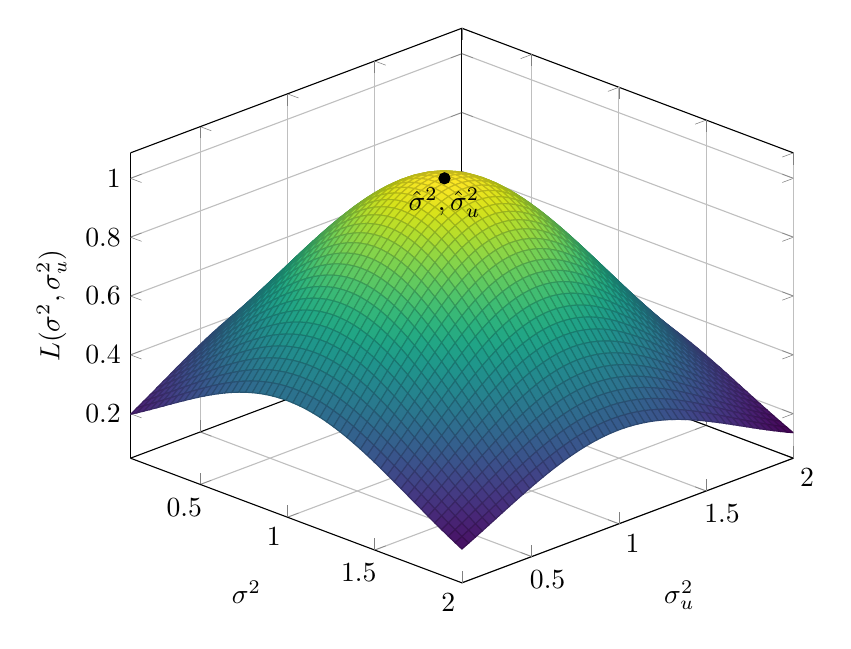
\begin{tikzpicture}
\begin{axis}[
    width=10cm,
    view={45}{30}, % Adjust viewing angle
    xlabel={\(\sigma^2\)},
    ylabel={\(\sigma_u^2\)},
    zlabel={\(L(\sigma^2, \sigma_u^2)\)},
    colormap/viridis,
    grid=major
]

% Define the likelihood surface
\addplot3[surf, domain=0.1:2, y domain=0.1:2, samples=50] 
{exp(-(x-1)^2 - (y-1)^2)};

% Annotate the peak
\addplot3[mark=*] coordinates {(1,1,1)} node[below] {\(\hat{\sigma}^2, \hat{\sigma}_u^2\)};

\end{axis}

\end{tikzpicture}
 \captionof{figure}{Illustration of MLE for two-parameters, $\sigma^2$ and $\sigma_u^2$ in a LMM. The MLE is the set of values for $\sigma^2$ and $\sigma_u^2$ at the peak of this surface, where the likelihood $L(\sigma^2, \sigma_u^2$) is maximized}
  \label{fig:MLEsurf}
 \end{tcolorbox}
 \end{wrapfigure}
Restricted Maximum Likelihood (REML) is a technique commonly used in mixed-effects models to obtain unbiased estimates of variance components, such as the variance of the random effects. Unlike standard Maximum Likelihood Estimation (MLE), which estimates both fixed and variance parameters simultaneously, REML focuses on estimating the variance components in a way that accounts for the loss of degrees of freedom due to the estimation of the fixed effects.

In mixed-effects models, the data consist of both fixed effects (such as population-level parameters) and random effects (such as group-specific deviations). The challenge with MLE is that it estimates both fixed effects and random effects variance simultaneously, leading to biased estimates of the variance components, especially when the sample size is small.

REML addresses this issue by ``restricting'' the likelihood to the random effects. This is achieved by conditioning on the fixed effects, thereby removing the influence of the fixed effects from the estimation of the random effects variance. Specifically, REML maximizes the likelihood of the residuals (the part of the data after accounting for the fixed effects), which provides a more accurate estimate of the variance components. By focusing on the residuals, REML ensures that the estimation of the variance components is unbiased, particularly in small sample sizes.

REML is especially useful when the goal is to obtain reliable estimates of the random effects variance $\sigma_u^2$ and $\sigma^2$, as it corrects for the bias that conventional MLE might introduce in small datasets.

The main distinction between REML and MLE lies in how they handle the estimation process. MLE estimates both fixed and random effects parameters simultaneously. REML, on the other hand, estimates the variance components based only on the residuals after the fixed effects are accounted for, which generally results in less bias, especially for the random effects variance. Overall, REML is the preferred method when the primary focus is on the random effects and variance components, as it provides unbiased estimates that are crucial for valid inference in mixed-effects models.

\section{Model Assumptions in LMM}
In Linear Mixed-Effects Models, several key assumptions underpin the validity of the model and the accuracy of the results. These assumptions include linearity, independence, normality, and homoscedasticity. Violations of these assumptions can lead to biased parameter estimates or incorrect conclusions. It's essential to assess whether these assumptions hold before interpreting the results of an LMM.

\subsection*{Linearity}
The linearity assumption posits that the relationship between the predictors (both fixed and random effects) and the response variable is linear. This means that the response $Y$ is modeled as a linear function of the predictors, with the fixed effects contributing to this linear relationship and the random effects accounting for variability between groups or clusters. Violations of this assumption can lead to misinterpretation of the effects of the predictors. For example, non-linear relationships might be overlooked, resulting in misleading conclusions about the strength or nature of the relationship between variables.

There are several ways to test whether the assumption of linearity is met. 
\begin{itemize}
\item \textbf{Residual vs. Fitted Plot}: This plot shows the residuals (errors) on the y-axis and the fitted values (predictions from the model) on the x-axis. A random scatter of points around zero indicates that the linearity assumption holds (.\\

If there are systematic patterns, such as curves or trends, this suggests that the relationship between predictors and the response might be nonlinear. If patterns appear, consider adding polynomial terms or using other nonlinear modeling approaches (e.g., splines, generalized additive models).

\begin{figure}[ht]
\centering
\begin{tikzpicture}
\begin{groupplot}[
  group style={group size=2 by 1, horizontal sep=2cm},
  width=6cm, height=5cm,
  xlabel={Fitted Values}, ylabel={Residuals},
  xmin=0, xmax=10, ymin=-10, ymax=10,
  axis lines=left, grid=both, enlargelimits=false
]

\nextgroupplot[title=Good Residual Plot]
\addplot+[only marks, mark=*, blue] table {
x y
1  1
2 -2
3  0.5
4 -1
5  1.5
6 -0.5
7  2
8 -2
9  0.5
10 -1
};

\addplot[red, thick] coordinates {(0,0) (10,0)};

\nextgroupplot[title=Nonlinear Pattern]
\addplot+[only marks, mark=*, blue] table {
x y
1  2
2  1.5
3  0
4 -2
5 -3
6 -2
7 -1
8  1
9  3
10 5
};

\addplot[red, thick] coordinates {(0,0) (10,0)};
\end{groupplot}
\end{tikzpicture}
\caption{Left: Random residuals suggest linearity. Right: Curved pattern suggests nonlinearity.}
\end{figure}

\item \textbf{Component Plus Residual (CERES) Plot}:  A more advanced plot that can detect both linearity and other functional form issues by adding fitted values for each predictor.
\end{itemize}

\subsection*{Independence}
The independence assumption states that the residual errors within each group are independent of each other. In other words, the errors for different observations within the same group should not be correlated. This assumption is critical because correlated errors violate the assumption of independent observations, which can bias both the estimation of fixed effects and the inference about variance components. However, the random effects are explicitly modeled as correlated within groups, which allows the model to account for this correlation at the group level. Residuals should not show patterns within groups, which could indicate a violation of the independence assumption.

There are several ways to test the independence assumption.
\begin{itemize}
\item \textbf{Durbin-Watson Test}: This test evaluates the autocorrelation of residuals. It is commonly used in time series models, but it can also be applied to check for residual dependence in mixed models. Values close to 2 suggest no autocorrelation, while values below 1 or above 3 indicate positive or negative autocorrelation, respectively.

\item \textbf{Plot of Residuals by Group}: If there is evidence of dependence within a group, such as a pattern in the residuals within certain levels of the grouping variable, it may indicate a violation of independence.

\item \textbf{Random Effects Variance}: If random effects are estimated to be large, this could suggest residual dependence, especially when they are unexplained by the model.
\end{itemize}

\subsection*{Normality}
Both the random effects $u$ and the residual errors $\epsilon$ are assumed to be normally distributed with mean zero. This assumption is crucial for statistical inference, as many of the inferential procedures (such as hypothesis testing and confidence interval estimation) rely on the normality of these components. If the residual errors or the random effects deviate significantly from normality, it may affect the precision of the estimates and the validity of statistical tests. Checking normality is important, especially for small sample sizes, as deviations can lead to larger biases or over-optimistic $p$-values.

There are several approaches to testing the normality assumption.
\begin{itemize}
\item \textbf{Q-Q Plot (Quantile-Quantile Plot)}: A Q-Q plot compares the quantiles of the residuals to the quantiles of a normal distribution. If the points fall approximately along a straight line, the residuals are likely normally distributed. Significant deviations from the straight line suggest departures from normality (e.g., heavy tails or skewness).

\item \textbf{Histogram of Residuals}: A histogram allows visual inspection of the distribution of residuals. For normality, the histogram should resemble a bell-shaped curve. If the shape is skewed or shows heavy tails, this indicates that the residuals are not normally distributed.

\item \textbf{Shapiro-Wilk Test / Anderson-Darling Test}: These statistical tests assess the normality of residuals. If the p-value is small (e.g., less than 0.05), the null hypothesis of normality is rejected, indicating non-normality.

\item \textbf{Normality of Random Effects}: You can also check the normality of random effects using a Q-Q plot or histogram of the random effects (if available), as random effects should follow a normal distribution by assumption.
\end{itemize}

\subsection*{Homoscedasticity}
The homoscedasticity assumption assumes that the variance of the residuals is constant across all groups. This means that the spread of residuals should be roughly the same across different levels of the grouping variable. If the residuals show unequal variance (a phenomenon known as heteroscedasticity), this can indicate that the model is mis-specified or that a transformation of the data may be necessary. Heteroscedasticity can lead to inefficiencies in the estimation process, and it can affect the reliability of the standard errors, making statistical inference problematic.

There are several ways to test the homoscedasticity assumption.
\begin{itemize} 
\item \textbf{Residual vs. Fitted Plot}: This plot can also be used to check for homoscedasticity. If the residuals fan out or contract as fitted values increase, it suggests heteroscedasticity (non-constant variance). Homoscedasticity would be indicated by a random scatter of residuals without any clear pattern.

\item \textbf{Scale-Location Plot (Spread-Location Plot)}: This plot shows the square root of the standardized residuals versus the fitted values. A horizontal line with equally spread points suggests homoscedasticity. If the plot shows a funnel shape (points spread out more as fitted values increase), this indicates heteroscedasticity.

\item \textbf{Breusch-Pagan Test}: This statistical test assesses the presence of heteroscedasticity by checking if the residual variance is related to the fitted values or other predictors. A significant result suggests heteroscedasticity.

\item \textbf{Levene’s Test}: A test that compares the variances between groups (useful in grouped data). It tests the null hypothesis that the variances are equal across groups, with significant p-values indicating a violation of homoscedasticity.
\end{itemize}

\begin{table}[h!]
\centering
\begin{tabular}{|l|l|}
\hline
\textbf{Assumption} & \textbf{Test Methods} \\
\hline
\textbf{Linearity} & Residual vs. Fitted Plot, Component Plus Residual (CERES) Plot, Polynomial Terms \\
\hline
\textbf{Independence} & Durbin-Watson Test, Plot of Residuals by Group, Random Effects Variance \\
\hline
\textbf{Normality} & Q-Q Plot, Histogram of Residuals, Shapiro-Wilk Test, Anderson-Darling Test \\
\hline
\textbf{Homoscedasticity} & Residual vs. Fitted Plot, Scale-Location Plot, Breusch-Pagan Test, Levene’s Test \\
\hline
\end{tabular}
\caption{Summary of Assumption Tests for Linear Mixed-Effects Models}
\end{table}

\section{A Complete Working Example}
In order to better understand LMM, let's consider an example, in this case a clinical psychology study that investigates the effectiveness of two therapeutic interventions (CBT vs. Mindfulness) on reducing anxiety levels in patients over six months. Measurements of anxiety scores are taken at three time points: baseline (0 months), mid-point (3 months), and endpoint (6 months).

Patients are nested within therapists, meaning each therapist treats multiple patients. The study includes:
\begin{itemize}
\item Fixed effects: \textbf{Type of therapy} (CBT or Mindfulness), \textbf{time} (baseline, 3 months, 6 months), and their interaction.

\item Random effects: \textbf{Therapist-level variability} (random intercepts for therapists).
\end{itemize}

The goal of the analysis is to assess whether the type of therapy and time have significant effects on anxiety scores while accounting for the clustering of patients within therapistss \dots but, before moving on, let's consider an important question \dots How is accounting for clustering of patients in therapists using LMM different from including therapists as an additional factor in regression or ANOVA? 
\vspace{.2cm}

\noindent \textit{They are fundamentally different approaches to handling grouped or hierarchical data.} Here’s a detailed comparison:

\noindent \textbf{ANOVA with Therapists as a Fixed Factor}
\begin{itemize}
\item In ANOVA, therapists are treated as a fixed factor, meaning each therapist is explicitly represented in the model.
\item This approach estimates a separate effect (mean adjustment) for each therapist, similar to including dummy variables for each therapist.
\item The number of parameters grows with the number of therapists, which can quickly become impractical if there are many therapists.
\item Assumes that the levels of the therapist factor are exhaustive or of specific interest (e.g., a finite set of therapists for whom you want individual comparisons).
\item Assumes homogeneity of variance across therapists, which may not reflect reality if therapists vary in effectiveness.
\item Results are specific to the therapists included in the study and cannot be generalized to a broader population of therapists.
\end{itemize}
\noindent \textbf{LMM with Therapists as a Random Effect}
\begin{itemize}
\item LMM treats therapists as a random effect, assuming the therapists in the dataset represent a sample from a larger population of therapists.
\item Instead of estimating a separate parameter for each therapist, the variability among therapists is modeled as a random variable with a mean of zero and a variance ($\sigma_u^2$).
\item LMM accounts for the clustering of patients within therapists without explicitly modeling each therapist as a fixed factor, making it more scalable and generalizable.
\item Captures the variability among therapists using a random-effects term, allowing for correlated observations within each therapist's group.
\item Results generalize to the population of therapists, as the random-effects structure assumes therapists are sampled from a larger population.
\end{itemize}

Now that we've considered why LMM may be more appropriate to help address the primary research question in this case, let's move on with the full example \dots

\subsection*{1. Set up the R environment}
Before getting started with this example, let's make sure that all of the required R packages are installed and loaded into the R environment.
\begin{mycode}[R]
# Load necessary libraries
install.packages("lme4")  # For mixed-effects models
install.packages("ggplot2")  # For visualization
install.packages("lmerTest")  # For p-values in mixed models

library(lme4)
library(ggplot2)
library(lmerTest)
\end{mycode}

\subsection*{2. Simulate Data}
Eventually, you will be using this example to conduct analyses with your own data, but for now, let's simulate some data to fit with our therapy study.
\begin{mycode}[R]
set.seed(123)
# Set parameters
n_patients <- 10          # Number of patients per therapist
n_therapists <- 5         # Number of therapists
time_points <- c(0, 3, 6) # Baseline, Mid-point, Endpoint

# Total number of observations
n_obs <- n_patients * n_therapists * length(time_points)

# Simulate therapist-level data
therapist_id <- rep(1:n_therapists, each = n_patients * 
     length(time_points) / n_therapists)
therapist_effects <- rep(rnorm(n_therapists, mean = 0, sd = 2), 
     each = n_patients * length(time_points) / n_therapists)

# Simulate patient-level data
therapy_type <- rep(c("CBT", "Mindfulness"), length.out = n_obs)
time <- rep(time_points, times = n_patients * n_therapists)

# Fixed effects: Therapy and time effects
cbt_effect <- ifelse(therapy_type == "CBT", -5, 0)
time_effect <- time * -0.8 # Decreasing anxiety over time
interaction_effect <- ifelse(therapy_type == "CBT", time * -0.8, 0) 
     # Greater improvement for CBT

# Generate anxiety scores
residual_error <- rnorm(n_obs, mean = 0, sd = 5) 
     # Residual error matches n_obs
anxiety_scores <- 50 + cbt_effect + time_effect + interaction_effect
      + therapist_effects + residual_error

# Create data frame
data <- data.frame(
  anxiety_scores = anxiety_scores,
  therapy_type = factor(therapy_type),
  time = factor(time, levels = time_points),
  therapist_id = factor(therapist_id)
)

# Display summary of the data
summary(data)
\end{mycode}
The above code will generate an R data frame containing simulated data from 50 patients nested in 10 therapists.  The random effects of therapist are drawn from a random normal distribution with a mean of zero and a standard deviation of 5.

\subsection*{3. Visualize the Data Before modeling}
As with ANY data analysis, it is important to generate some visualizations of your data before you start conducting your statistical analyses.  The code below illustrates how you might review the raw data using a grouped longitudinal dot plot. This type of visualization is often used to depict changes in response variables over time across different groups or conditions. It could also be referred to as a time-series scatter plot by group.
\begin{mycode}[R]
# Plot anxiety scores over time by therapy type
ggplot(data, aes(x = time, y = anxiety_scores, color = therapy_type)) + 
    geom_point(position = position_jitter(width = 0.1, height = 0)) + 
    geom_smooth(method = "loess", se = FALSE) +
    labs(title = "Anxiety Scores Over Time by Therapy Type",
         x = "Time (Months)", y = "Anxiety Score") +
    theme_minimal()
\end{mycode} 

\mywrapfigure{Example of a Grouped Longitudinal Dot Plot}{.5\linewidth}{LinearMixedModels/Figures/LMMclinicalPlot1.png}{This plot depicts changes in anxiety over time across the CBT and Mindfullness conditions.}{fig:CBTMindfullnessRaw}
\FloatBarrier % Fix floating issues

\subsection*{4: Fit the Linear Mixed-Effects Model}
In this analysis, we will fit a LMM to account for the hierarchical structure of the data, where patients are nested within therapists. The model includes random intercepts for therapists, which allow each therapist to have their own baseline anxiety level, reflecting unmeasured therapist-level differences that might influence patient outcomes. Fixed effects are included for therapy type (CBT vs. Mindfulness), time (baseline, mid-point, and endpoint), and their interaction. The main effects for therapy type and time capture the overall differences between therapies and the progression of anxiety scores over time, respectively. The interaction term allows us to assess whether the rate of change in anxiety scores over time differs between the two therapy types. By including random intercepts, the LMM accounts for the clustering of patients within therapists, providing more accurate estimates of fixed effects and properly partitioning variance between therapists and patients.

\begin{tcolorbox}[every float=\centering, drop shadow,     title=R Code]
\begin{verbatim}
# Fit the model
model <- lmer(anxiety_scores ~ therapy_type * time + 
     (1 | therapist_id), data = data)

# Display summary
summary(model)    \end{verbatim}
\tcblower
\begin{codeblock}{Fitting the LMM and displaying a summary of the result.}\label{code:LMMfit}\end{codeblock}
\end{tcolorbox}
\clearpage

 The output (i.e., summary) of this model fit will contain several sections summarizing measures of model fit and the fit statistics. Each section is illustrated and explained in the table below.

 
 \small{
\begin{longtable}{|p{\linewidth}|}
\hline
\rowcolor{gray!10}
\textbf{Output:} \newline 
Linear mixed model fit by REML. t-tests use Satterthwaite's method [`lmerModLmerTest'] \newline 
Formula: anxiety\_scores \textasciitilde{} therapy\_type * time + (1 | therapist\_id) \newline
Data: data\\
\hline
\textbf{Explanation:} \newline 
This part of the output provides key information about how the linear mixed model (LMM) was fit, how statistical tests were performed, and specifies the LMM formula. \newline
\begin{itemize}
\item Note that the model was fit using REML (default).  If you prefer to use maximum likelihood (ML), you can add the REML=false argument when fitting the model. 
\item The fixed effects include therapy type, time, and their interaction. The random effects term \texttt{(1 | therapist\_id)} allows each therapist to have a random intercept, accounting for between-therapist variability.
\item The fixed-effect coefficient significance is tested using Satterthwaite’s approximation to calculate degrees of freedom. This method adjusts the degrees of freedom to account for the hierarchical structure of the data (e.g., clustering by therapists), providing more accurate p-values for fixed effects.
\item The output also shows the class of the model object created by the lmer() function in the lmerTest package, which extends the functionality of the lme4 package to include p-value calculations for fixed effects.\end{itemize} \\
\hline
\rowcolor{gray!10}
\textbf{Output:} \newline 
REML criterion at convergence: 877.6 \\ 
\hline
\textbf{Explanation:} \newline 
The REML criterion is a measure of model fit. Lower values indicate a better fit. \begin{itemize}
\item The REML convergence criterion itself is not typically interpreted directly as ``good'' or ``bad.'' Instead, it is a numerical value used to determine whether the optimization algorithm has successfully converged during the fitting process of a LMM. 
\item Lower values of the REML criterion indicate a better fit, but only in a relative sense. For example, when comparing nested models (e.g., using likelihood ratio tests), the model with the lower REML criterion is the better fit. The absolute value of the REML criterion depends on the scale of the outcome variable, the size of the dataset, and the complexity of the model (number of fixed and random effects).\end{itemize}\\
\hline
\rowcolor{gray!10}
\textbf{Output:} \newline  
\begin{tabular}{rrrrrr}
Scaled residuals: & Min & 1Q & Median & 3Q & Max \\
& -2.31120 & -0.73545 & -0.05507 & 0.64579 & 2.36512 \\
\end{tabular} \\
\hline
\textbf{Explanation:} \newline 
Scaled residuals provide a summary of the model's residuals (differences between observed and predicted values). They are standardized for interpretation, and extreme values may indicate outliers or model issues. \\
\hline
\rowcolor{gray!10}
\textbf{Output:} \newline 
\begin{tabular}{lrrrr}
Random effects: & \textbf{Groups} & \textbf{Name} & \textbf{Variance} & \textbf{Std.Dev.} \\
& therapist\_id & (Intercept) & 0.5635 & 0.7507 \\
& & Residual & 22.3566 & 4.7283 \\
\end{tabular}\newline
Number of obs: 150, groups: therapist\_id, 5 \\ 
\hline
\textbf{Explanation:} \newline 
The random intercept variance for therapists (\texttt{0.5635}) reflects differences in baseline anxiety scores across therapists. The residual variance (\texttt{22.3566}) represents unexplained within-patient variability in anxiety scores. \newline
There are 150 total observations (patients across time points) nested within 5 therapist groups. This clustering is modeled using random effects.\\
\hline
\rowcolor{gray!10}
\textbf{Output:} \newline 
\begin{tabular}{lrrrrrc}
\textbf{Fixed effects:} & \textbf{Estimate} & \textbf{Std. Error} & \textbf{df} & \textbf{t value} & \textbf{Pr(>|t|)} \\
\hline
(Intercept) & 44.47 & 1.003 & 48.067 & 44.322 & < 2e-16 & ***\\
therapy\_typeMindfulness & 4.847 & 1.337 & 140.000 & 3.624 & 0.0004 & ***\\
time3 & -3.374 & 1.337 & 140.000 & -2.523 & 0.0127 & * \\
time6 & -8.805 & 1.337 & 140.000 & -6.584 & 8.55e-10 & *** \\
therapy\_typeMindfulness:time3 & 3.551 & 1.891 & 140.000 & 1.878 & 0.0625 & . \\
therapy\_typeMindfulness:time6 & 4.359 & 1.891 & 140.000 & 2.305 & 0.0226 & * \\
\hline
\end{tabular}\newline
Signif. codes:  0 ‘***’ 0.001 ‘**’ 0.01 ‘*’ 0.05 ‘.’ 0.1 ‘ ’ 1 \\ 
\hline
\textbf{Explanation:} \newline 
\begin{itemize}
\item The intercept (\texttt{47.476}) represents the baseline anxiety score for CBT at time 0. Therapy type and time effects capture differences in anxiety scores due to therapy type (Mindfulness vs. CBT) and progression over time. Significant effects (\texttt{time6}, \(p < 0.001\)) suggest lower anxiety scores at 6 months.
\item In typical statistical output from models, like those produced by R, the ``time0'' category (often the baseline or reference level for a factor) is not explicitly listed in the fixed effects table. This happens because the reference level is implicitly represented by the intercept term.  When you have categorical variables like therapy\_type and time, the model automatically chooses one level of each factor as a reference. In this case, the model has probably chosen therapy\_type with CBT and time0 as the reference levels.
\item The interaction terms test whether the effect of time differs between therapy types. Non-significant results (\(p > 0.05\)) indicate no strong evidence that the change over time depends on therapy type.\end{itemize}\\
\hline
\rowcolor{gray!10}
\textbf{Output:} \newline 
\begin{tabular}{lrrrrr}
\textbf{Correlation of Fixed Effects:} & \textbf{(Intr)} & \textbf{thrp\_M} & \textbf{time3} & \textbf{time6} & \textbf{th\_M:3} \\
\hline
thrp\_typeMn & -0.666 & & & & \\
time3 & -0.666 & 0.500 & & & \\
time6 & -0.666 & 0.500 & 0.500 & & \\
thrp\_typeM:3 & 0.471 & -0.707 & -0.707 & -0.354 & \\
thrp\_typeM:6 & 0.471 & -0.707 & -0.354 & -0.707 & 0.500 \\
\hline
\end{tabular} \\ 
\hline
\textbf{Explanation:} \newline 
\begin{itemize}
\item The correlation matrix shows relationships between fixed effect estimates. For example, \texttt{thrpy\_typMn} (therapy type) is negatively correlated with the intercept (\texttt{-0.666}). High correlation between two fixed effects suggests that the two predictors share a lot of common information, potentially leading to multicollinearity (which can distort the interpretation of the coefficients). 
\item For example, thrp\_typeMn and time3: The correlation here is 0.500, meaning there is a moderate positive relationship between the effect of therapy\_typeMindfulness and time3. This suggests that the higher the effect of therapy\_typeMindfulness, the stronger the effect of time3, and vice versa.
\item High correlations between predictors (such as thrp\_typeMn, time3, time6, etc.) might suggest collinearity issues. In your case, correlations like -0.666 between the intercept and the other variables, and 0.500 between some variables, suggest that some of the predictors share a fair amount of common variance. While not necessarily problematic, you should check whether these correlations lead to multicollinearity issues (which can inflate standard errors and make coefficient estimates unstable).\end{itemize}\\
\hline
\caption{Summary of the LMM fit}
\label{table:LMMfit1}
\end{longtable}
}

\subsection*{Reporting LMM Results}
Once you have fit the LMM, it is important to consider how you will report the results. While there is no strict APA standard for reporting linear mixed models, it is important to provide enough detail about the model specification and results that the reader can evaluate the model specification, fit, and statistical results.  

For example \dots ``We conducted a linear mixed model analysis in R, with [dependent variable] as the outcome variable, [fixed effects] as fixed effects, and [random effects] as random effects. The model specification was: [DV] ~ [fixed effects] + (1|random effects). The analysis revealed a significant effect of Therapy Type ($\beta$ = 4.85, SE = 1.00, $t$(140) = 3.62, $p$ < .001, 95\% CI [2.23, 7.47]) and a significant Time × Therapy Type interaction at six months ($\beta$ = 4.36, SE = 1.89, $t$(140) = 2.31, $p$ = .022, 95\% CI [0.65, 8.07]). The random effect of participant accounted for 1.2\% of the total variance.''

Note that the confidence intervals and variance accounted for ($R^2$) are not part of the default output in R.  However, these values can easily be computed from the model estimated by the lme4 package using the \texttt{confint()} function.
\[95\%CI=\begin{cases}confint(model, method="Wald")  \# \text{For fixed effects only} \\
confint(model, method="profile") \# \text{For both fixed and random effects}\\
confint(model, method="boot") \# \text{Bootstrap method}\end{cases}
\]

In order to compute the variance accounted for ($R^2$), you will likely need to install and load the ``performance'' package.  Calling the \texttt{r2()} function will then yield the conditional and the marginal $R^2$ (see code block below).  The conditional $R^2$ includes both fixed and random effects and the marginal $R^2$ only accounts for the fixed effects.  The percent variance accounted for by only the random effects is the difference between the two, $R_{conditional}^2 - R_{marginal}^2$.
\begin{tcolorbox}[every float=\centering, drop shadow,     title=R Code]
\begin{verbatim}
# Install additional packages \% variance accounted for
install.package(``performance'')
library(performance)

# Get percent variance accounted for
> r2(model)
	Conditional R2: 0.513
	Marginal R2: 0.501

# Get 95\% confidence intervals
> confint(model, method="profile")
                                    2.5 \%     97.5 \%
.sig01                          0.0000000  2.0622077
.sigma                          4.1585789  5.2367328
(Intercept)                    42.5573209 46.3951265
therapy_typeMindfulness         2.2543649  7.4398386
time3                          -5.9670212 -0.7815476
time6                         -11.3975347 -6.2120611
therapy_typeMindfulness:time3  -0.1156872  7.2176799
therapy_typeMindfulness:time6   0.6924522  8.0258193
 \end{verbatim}
\tcblower
\begin{codeblock}{Getting the $R^2$ and 95\% CIs from the LMM model.}\label{code:LMMci}\end{codeblock}
\end{tcolorbox}


\section{Visualizing the Results of a LMM}
Linear mixed effect models can be visualized in several effective ways to understand both fixed and random effects. Here are the key visualization approaches:
\printglossary[type=datacollection,style=twocolumn]
%\printglossary
%\glsresetall
\newpage
\bibliographystyle{apalike}
\renewcommand{\bibname}{References}
\bibliography{bibliography}

